\documentclass[oneside,openright,titlepage,numbers=noenddot,headinclude,
                footinclude=true,cleardoublepage=empty,
                BCOR=5mm,paper=a4,fontsize=11pt]{book} 
                
%%%%%%%%%%%%%%%%%%%%%%%%%%%%%%%%%%%%%%%%%
% Thesis Configuration File
%
% The main lines to change in this file are in the DOCUMENT VARIABLES
% section, the rest of the file is for advanced configuration.
%
%%%%%%%%%%%%%%%%%%%%%%%%%%%%%%%%%%%%%%%%%

%----------------------------------------------------------------------------------------
%	DOCUMENT VARIABLES
%	Fill in the lines below to enter your information into the thesis template
%	Each of the commands can be cited anywhere in the thesis
%----------------------------------------------------------------------------------------

% Remove drafting to get rid of the '[ Date - classicthesis version 4.0 ]' text at the bottom of every page
\PassOptionsToPackage{eulerchapternumbers,drafting, pdfspacing, subfig,beramono,eulermath,parts}{classicthesis}
% Available options: drafting parts nochapters linedheaders eulerchapternumbers beramono eulermath pdfspacing minionprospacing tocaligned dottedtoc manychapters listings floatperchapter subfig
% Adding 'dottedtoc' will make page numbers in the table of contents flushed right with dots leading to them

\newcommand{\myTitle}{Diccionarios de Representaci\'on Dispersa para Codificaci\'on de Video usando Caracter\'isticas Perceptuales\xspace}
\newcommand{\mySubtitle}{}
\newcommand{\myDegree}{}
\newcommand{\myNameA}{Ing. Augusto G\'omez Vinasco\xspace}
\newcommand{\myProf}{}
\newcommand{\myOtherProf}{}
\newcommand{\mySupervisor}{Mar\'ia Patricia Trujillo, Ph.D.\xspace}
\newcommand{\myFaculty}{Facultad de Ingenier\'ia \xspace}
\newcommand{\myDepartment}{Escuela de Ingenier\'ia de Sistemas y Computaci\'on \xspace}
\newcommand{\myUni}{Universidad del Valle\xspace}
\newcommand{\myLocation}{Cali, Colombia\xspace}
\newcommand{\myTime}{Enero 2017\xspace}
\newcommand{\myVersion}{version 2.0\xspace}

%----------------------------------------------------------------------------------------
%	USEFUL COMMANDS
%----------------------------------------------------------------------------------------

\newcommand{\ie}{i.\,e.}
\newcommand{\Ie}{I.\,e.}
\newcommand{\eg}{e.\,g.}
\newcommand{\Eg}{E.\,g.} 



\newcounter{dummy} % Necessary for correct hyperlinks (to index, bib, etc.)
\providecommand{\mLyX}{L\kern-.1667em\lower.25em\hbox{Y}\kern-.125emX\@}

%----------------------------------------------------------------------------------------
%	PACKAGES
%----------------------------------------------------------------------------------------

\usepackage{lipsum} % Used for inserting dummy 'Lorem ipsum' text into the template

\usepackage{multirow}
\usepackage{multicol}
\usepackage{algorithm}
\usepackage{algpseudocode}
\usepackage{url}
\usepackage[inline]{enumitem}
\usepackage{array}
\usepackage[dottedtoc]{classicthesis}
\usepackage{colortbl}
\usepackage{longtable}
\usepackage{bm}

%------------------------------------------------
 
\PassOptionsToPackage{latin9}{inputenc} % latin9 (ISO-8859-9) = latin1+"Euro sign"
\usepackage[utf8]{inputenc}
 
%------------------------------------------------
\usepackage{float}
%------------------------------------------------

%\PassOptionsToPackage{ngerman,american}{babel}  % Change this to your language(s)
% Spanish languages need extra options in order to work with this template
\PassOptionsToPackage{spanish,es-lcroman,es-tabla}{babel}
\usepackage{babel}

%------------------------------------------------			

\PassOptionsToPackage{square,numbers}{natbib}
 \usepackage{natbib}
 
 %------------------------------------------------

%\PassOptionsToPackage{fleqn}{amsmath} % Math environments and more by the AMS 
 \usepackage{amsmath}
 
 %------------------------------------------------

\PassOptionsToPackage{T1}{fontenc} % T2A for cyrillics
\usepackage{fontenc}

%------------------------------------------------

\usepackage{xspace} % To get the spacing after macros right

%------------------------------------------------

\usepackage{mparhack} % To get marginpar right

%------------------------------------------------

\usepackage{fixltx2e} % Fixes some LaTeX stuff 

%------------------------------------------------

\PassOptionsToPackage{smaller}{acronym} % Include printonlyused in the first bracket to only show acronyms used in the text
\usepackage{acronym} % nice macros for handling all acronyms in the thesis

%------------------------------------------------

%\renewcommand*{\acsfont}[1]{\textssc{#1}} % For MinionPro
%\renewcommand{\bflabel}[1]{{#1}\hfill} % Fix the list of acronyms

%------------------------------------------------

\PassOptionsToPackage{pdftex}{graphicx}
\usepackage{graphicx} 
\usepackage{epstopdf}

%----------------------------------------------------------------------------------------
%	FLOATS: TABLES, FIGURES AND CAPTIONS SETUP
%----------------------------------------------------------------------------------------

\usepackage{tabularx} % Better tables
\setlength{\extrarowheight}{3pt} % Increase table row height
\newcommand{\tableheadline}[1]{\multicolumn{1}{c}{\spacedlowsmallcaps{#1}}}
\newcommand{\myfloatalign}{\centering} % To be used with each float for alignment
\usepackage{caption}
\captionsetup{format=hang,font=small}
\usepackage{subfig}  

%----------------------------------------------------------------------------------------
%	CODE LISTINGS SETUP
%----------------------------------------------------------------------------------------

\usepackage{listings} 
%\lstset{emph={trueIndex,root},emphstyle=\color{BlueViolet}}%\underbar} % for special keywords
\lstset{language=[LaTeX]Tex, % Specify the language for listings here
keywordstyle=\color{RoyalBlue}, % Add \bfseries for bold
basicstyle=\small\ttfamily, % Makes listings a smaller font size and a different font
%identifierstyle=\color{NavyBlue}, % Color of text inside brackets
commentstyle=\color{Green}\ttfamily, % Color of comments
stringstyle=\rmfamily, % Font type to use for strings
numbers=left, % Change left to none to remove line numbers
numberstyle=\scriptsize, % Font size of the line numbers
stepnumber=5, % Increment of line numbers
numbersep=8pt, % Distance of line numbers from code listing
showstringspaces=false, % Sets whether spaces in strings should appear underlined
breaklines=true, % Force the code to stay in the confines of the listing box
%frameround=ftff, % Uncomment for rounded frame
frame=single, % Frame border - none/leftline/topline/bottomline/lines/single/shadowbox/L
belowcaptionskip=.75\baselineskip % Space after the "Listing #: Desciption" text and the listing box
}

%----------------------------------------------------------------------------------------
%	HYPERREFERENCES
%----------------------------------------------------------------------------------------

\PassOptionsToPackage{pdftex,hyperfootnotes=false,pdfpagelabels}{hyperref}
\usepackage{hyperref}  % backref linktocpage pagebackref
\pdfcompresslevel=9
\pdfadjustspacing=1

\hypersetup{
% Uncomment the line below to remove all links (to references, figures, tables, etc)
%draft, 
colorlinks=true, linktocpage=true, pdfstartpage=3, pdfstartview=FitV,
% Uncomment the line below if you want to have black links (e.g. for printing black and white)
%colorlinks=false, linktocpage=false, pdfborder={0 0 0}, pdfstartpage=3, pdfstartview=FitV, 
breaklinks=true, pdfpagemode=UseNone, pageanchor=true, pdfpagemode=UseOutlines,
plainpages=false, bookmarksnumbered, bookmarksopen=true, bookmarksopenlevel=1,
hypertexnames=true, pdfhighlight=/O, urlcolor=webbrown, linkcolor=RoyalBlue, citecolor=webgreen,
%------------------------------------------------
% PDF file meta-information
pdftitle={\myTitle},
pdfauthor={\textcopyright\ \myNameA, \myUni, \myFaculty},
pdfsubject={},
pdfkeywords={},
pdfcreator={pdfLaTeX},
pdfproducer={LaTeX with hyperref and classicthesis}
%------------------------------------------------
}   

%----------------------------------------------------------------------------------------
%	BACKREFERENCES
%----------------------------------------------------------------------------------------

\usepackage{ifthen} % Allows the user of the \ifthenelse command
\newboolean{enable-backrefs} % Variable to enable backrefs in the bibliography
\setboolean{enable-backrefs}{false} % Variable value: true or false

\newcommand{\backrefnotcitedstring}{\relax} % (Not cited.)
\newcommand{\backrefcitedsinglestring}[1]{(Cited on page~#1.)}
\newcommand{\backrefcitedmultistring}[1]{(Cited on pages~#1.)}
\ifthenelse{\boolean{enable-backrefs}} % If backrefs were enabled
{
\PassOptionsToPackage{hyperpageref}{backref}
\usepackage{backref} % to be loaded after hyperref package 
\renewcommand{\backreftwosep}{ and~} % separate 2 pages
\renewcommand{\backreflastsep}{, and~} % separate last of longer list
\renewcommand*{\backref}[1]{}  % disable standard
\renewcommand*{\backrefalt}[4]{% detailed backref
\ifcase #1 
\backrefnotcitedstring
\or
\backrefcitedsinglestring{#2}
\else
\backrefcitedmultistring{#2}
\fi}
}{\relax} 

%----------------------------------------------------------------------------------------
%	AUTOREFERENCES SETUP
%	Redefines how references in text are prefaced for different 
%	languages (e.g. "Section 1.2" or "section 1.2")
%----------------------------------------------------------------------------------------

\makeatletter
\@ifpackageloaded{babel}
{
\addto\extrasamerican{
\renewcommand*{\figureautorefname}{Figure}
\renewcommand*{\tableautorefname}{Table}
\renewcommand*{\partautorefname}{Part}
\renewcommand*{\chapterautorefname}{Chapter}
\renewcommand*{\sectionautorefname}{Section}
\renewcommand*{\subsectionautorefname}{Section}
\renewcommand*{\subsubsectionautorefname}{Section}
}
\addto\extrasngerman{
\renewcommand*{\paragraphautorefname}{Absatz}
\renewcommand*{\subparagraphautorefname}{Unterabsatz}
\renewcommand*{\footnoteautorefname}{Fu\"snote}
\renewcommand*{\FancyVerbLineautorefname}{Zeile}
\renewcommand*{\theoremautorefname}{Theorem}
\renewcommand*{\appendixautorefname}{Anhang}
\renewcommand*{\equationautorefname}{Gleichung}
\renewcommand*{\itemautorefname}{Punkt}
}
\providecommand{\subfigureautorefname}{\figureautorefname} % Fix to getting autorefs for subfigures right
}{\relax}
\makeatother


\newcolumntype{C}[1]{>{\centering\let\newline\\\arraybackslash\hspace{0pt}}m{#1}}

%----------------------------------------------------------------------------------------

\usepackage{classicthesis} 

%----------------------------------------------------------------------------------------
%	CHANGING TEXT AREA 
%----------------------------------------------------------------------------------------

%\linespread{1.05} % a bit more for Palatino
%\areaset[current]{312pt}{761pt} % 686 (factor 2.2) + 33 head + 42 head \the\footskip
%\setlength{\marginparwidth}{7em}%
%\setlength{\marginparsep}{2em}%

%----------------------------------------------------------------------------------------
%	USING DIFFERENT FONTS
%----------------------------------------------------------------------------------------

%\usepackage[oldstylenums]{kpfonts} % oldstyle notextcomp
%\usepackage[osf]{libertine}
%\usepackage{hfoldsty} % Computer Modern with osf
%\usepackage[light,condensed,math]{iwona}
%\renewcommand{\sfdefault}{iwona}
%\usepackage{lmodern} % <-- no osf support :-(
%\usepackage[urw-garamond]{mathdesign} <-- no osf support :-(

\usepackage[colorinlistoftodos]{todonotes}




\cfoot{\pagemark}

\begin{document}

\frenchspacing % Reduces space after periods to make text more compact
\raggedbottom % Makes all pages the height of the text on that page

\pagenumbering{roman} 
\pagestyle{plain}

%\begin{titlepage}

%\begin{addmargin}[1cm]{3cm}
\begin{center}
\large

\hfill
\vfill

\begingroup
\color{Maroon}\spacedallcaps{\myTitle} \\ \bigskip % Thesis title
\endgroup

\spacedlowsmallcaps{\myNameA} \\% Your name
%\spacedlowsmallcaps{\myCodeA} \\ 


\vfill
Directora:
\spacedlowsmallcaps{\mySupervisor}
\vfill


\includegraphics[width=3cm]{images/logo.eps} \\ \medskip % Picture

%\mySubtitle \\ \medskip % Thesis subtitle
%\myDegree \\
\myDepartment \\
\myFaculty \\
\myUni \\ \bigskip

\myTime\ %-- \myVersion  Time and version

\vfill

\end{center}
%\end{addmargin}

\end{titlepage}
%\clearpage\pagestyle{scrheadings}
%\clearpage% Table of Contents - List of Tables/Figures/Listings and Acronyms

\refstepcounter{dummy}

\pdfbookmark[1]{\contentsname}{tableofcontents} % Bookmark name visible in a PDF viewer

\setcounter{tocdepth}{2} % Depth of sections to include in the table of contents - currently up to subsections

\setcounter{secnumdepth}{3} % Depth of sections to number in the text itself - currently up to subsubsections

\manualmark
\markboth{\spacedlowsmallcaps{\contentsname}}{\spacedlowsmallcaps{\contentsname}}
\tableofcontents 
\automark[section]{chapter}
\renewcommand{\chaptermark}[1]{\markboth{\spacedlowsmallcaps{#1}}{\spacedlowsmallcaps{#1}}}
\renewcommand{\sectionmark}[1]{\markright{\thesection\enspace\spacedlowsmallcaps{#1}}}

\clearpage

\begingroup 
\let\clearpage\relax
\let\cleardoublepage\relax
\let\cleardoublepage\relax

%----------------------------------------------------------------------------------------
%	List of Figures
%----------------------------------------------------------------------------------------

\refstepcounter{dummy}
%\addcontentsline{toc}{chapter}{\listfigurename} % Uncomment if you would like the list of figures to appear in the table of contents
\pdfbookmark[1]{\listfigurename}{lof} % Bookmark name visible in a PDF viewer

\listoffigures

\vspace*{8ex}
\newpage

%----------------------------------------------------------------------------------------
%	List of Tables
%----------------------------------------------------------------------------------------

\refstepcounter{dummy}
%\addcontentsline{toc}{chapter}{\listtablename} % Uncomment if you would like the list of tables to appear in the table of contents
\pdfbookmark[1]{\listtablename}{lot} % Bookmark name visible in a PDF viewer

\listoftables
        
\vspace*{8ex}

\endgroup

\cleardoublepage
\pagenumbering{arabic} 
\clearpage\chapter{Problem}
\label{chap:problem}

\section{Problem Statement}

The advence in new video technologies suggest new resolution size (
4k(3840$\times$2160px) or 8k(7680$\times$4320px)), an increasing in the frame
rate (60fps - 120 fps) and an increasing in the  color representation formats
(10 bits and 12 bits). Moreover, the advance in differents technologies, as
cloud computing, have promoted the use of video-based services, such as 
streaming, video-conference, video-on-demand, IPTV, broadcasting, among others,
which have generated an significant increment in the amount of information
neccesary for representing a video. By example, Table \ref{fig:youtube} shows
the bit-rate required for representing a live streaming video through YouTube
with a specific resolution\footnote{\url{https://support.google.com/youtube/answer/2853702}}.

\begin{table}[!h]
\centering
\begin{tabular}{|c|c|c|}
\hline
\textbf{Resolution} & \textbf{Bit-rate Min (Kbps)} & \textbf{bit-rate Max (Kbps)} \\
\hline
2560$\times$1440$@$60 & 9000 & 18000 \\
\hline
2560$\times$1440$@$30 &  6000 & 13000  \\
\hline
1920$\times$1080$@$60 & 4500 & 9000\\
\hline
1920$\times$1080 & 3000 & 6000 \\
\hline
\end{tabular}
\caption{Bit-rate requirements for some video resolutions in live
streaming video for YouTube}
\label{fig:youtube}
\end{table}

in addition to high bit-rate requeriments, there are limitations in bandwidth in
some geographic regions, for example, Latin America has a internet speed
connection of 7.26 Mbps on average for fixed networks and 4 Mbps for mobile
networks on average \cite{cepal}. The high bit-rates and bandwidth limitations
involve continuous efforts to maximize the coding efficiency, i.e. reducing the
bit rate, keeping the video quality.

The conventional video encoders, as HEVC or VP9, use differents techniques for
exploting the statistical, psychovisual and coding redundancies present in a
video. This techniques have been widely deployed and now is neccesary to adapt
to conventional video encoders others strategies that can to maximize the
compression capacity. 

The sparse representation emerge as alternative for improving the coding
eficiency, exploiting the sparsity propierties of signals for compressing with a
small amount of samples in terms of a base called dictionary. The sparse
representation is generated solving an optimization problem of $\ell_p$-norm of
sparse vector, such that lineal combination between the dictionary and the
sparse vector aproximate the original signal. A key problem of sparse
representation is the dictionary selection, because a good dictionary can to
guarantee a better signal reconstruction. The dictionary can be constructed with
samples extracted directly of the signal or can be trained for adapt it to
signal. The training process of dictionary consists of initialization step and
an iterative process of updating based on optimization problem of $\ell_p$-norm.
The updating process depends on convergence of the problem and should be
searched strategies for increasing the speed of convergence, due to the
dictionary training aggregate a significant computational cost.



\section{Problem Formulation}
How to optimize the training process of the dictionary of modeling of sparse
representation for video coding?

\section{Objectives}
\subsection{General Objective}
To Optimize the training process of dictionary for modelling the sparse
representation for video coding

\subsection{Specific objectives}
\begin{itemize}
\item Reducing the training time of a dictionary for sparse
representation based on video signals samples Reducir el tiempo de entrenamiento
\item Design a training model of dictionary that integrate perceptual coding
methods
\item To minimize the reconstruction error of the video signal when
using the traning model designed
\item To implement the designed model adapting to video coding
software 
\end{itemize}


\clearpage\chapter{Marco Conceptual}
\label{chap:background}

\section{Codificaci\'on de Video}
Un problema de los videos sin compresi\'on (RAW) ha sido el almacenamiento y la transmisi\'on, debido al gran n\'umero de bits que contienen. Por esta raz\'on se requiere el uso de t\'ecnicas de compresi\'on para reducir el n\'umero de bits que representan el video. La codificaci\'on de video toma ventaja de tres tipos de redundancias  presentes en un video \cite{motion}:
\begin{itemize}
    \item \textbf{Redundancia estad\'istica:} se refiere a la alta correlaci\'on espacial entre pixeles en un frame y la correlaci\'on temporal entre pixeles co-localizados en frames consecutivos.
    \item \textbf{Redundancia psicovisual:} debido a las limitaciones y caracter\'isticas del sistema visual humano se puede eliminar informaci\'on que no se distingue.
    \item \textbf{Redundancia de C\'odigo:} se produce por la repetici\'on de s\'imbolos que representan la informaci\'on de video.
\end{itemize}

Los est\'andares de codificaci\'on implementan un conjunto de herramientas para explotar estas redundancias de un video. La figura \ref{codec} presenta un diagrama de bloques de un est\'andar de codificaci\'on de video, el cual tiene dos m\'odulos principales, el codificador y el decodificador.
	
\begin{figure}[!h]
\centering
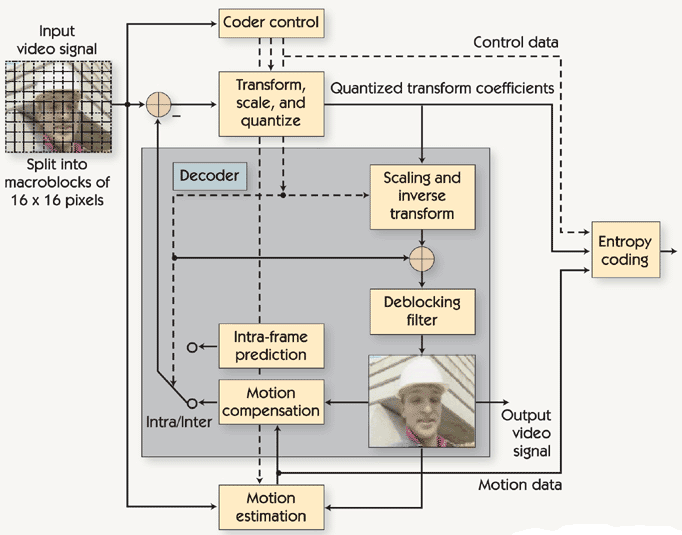
\includegraphics[width=0.6\textwidth]{images/codec.png}
\caption[Diagrama de Bloques de un est\'andar de codificaci\'on de video]{Diagrama de Bloques de un est\'andar de codificaci\'on de video
\scriptsize{\textbf{Fuente:} \url{http://www.eetimes.com/document.asp?doc_id=1272639}}}
\label{codec}
\end{figure}

Los codificacores de video consiste de tres elementos principales, los cuales explotan cada una de las redundancias:
\begin{itemize}
	\item El \textbf{predictor} que realiza una predicci\'on intra-frame para explotar la correlaci\'on espacial y una predicci\'on inter-frame para explotar la correlaci\'on temporal. 
	\item El \textbf{cuantizador} reduce la exactitud de las representaciones del predictor mediante un criterio de fidelidad para eliminar la redundancia psicovisual.
	\item La \textbf{codificaci\'on de entrop\'ia} reduce el n\'umero de s\'imbolos necesarios para representar el video aprovechando la similaridad de los s\'imbolos resultantes de la cuantizaci\'on.
\end{itemize}

Los codificadores realizan el proceso inverso de cada uno de los elementos para reconstruir la informaci\'on codificada. En el proceso de reconstrucci\'on se presenta p\'erdida de la informaci\'on debido a la eliminaci\'on o tranformaci\'on de la informaci\'on original en el codificador.

\section{Compressive Sensing}

La p\'erdida de informaci\'on en la codificaci\'on de video esta relacionada a dos suposiciones: la primera es la imperfecci\'on del HVS (sensitividad) y la segunda est\'a relacionada a propiedades espec\'ificas de la se\~nal en cierto dominio transformado. El objetivo de \textit{compressed sensing} (CS) es reconstuir una se\~nal usando un peque\~no conjunto de muestras de la se\~nal \cite{compressive}. Uno de los principales requerimientos que se deben satisfacer para aplicar t\'ecnicas de CS es la representaci\'on dispersa. 

\subsection{Representaci\'on dispersa}

Consideramos una se\~nal $\boldsymbol{x} \in \mathbb{R}^N$. Dada una matriz de base ortonormal $\boldsymbol{B} \in \mathbb{R}^{N \times N}$, donde sus columnas son lo elementos base $ \{\boldsymbol{b}_i\}_{i=1}^N$, $\boldsymbol{x}$ puede ser representada en t\'erminos de este base como:
\begin{center}
\begin{equation}
\boldsymbol{x}=\sum \limits_{i=1}^{N} \boldsymbol{\alpha}_i \boldsymbol{b}_i
\end{equation}
\end{center}
donde $\boldsymbol{\alpha}$ es un vector de coeficientes  y $\boldsymbol{b}_i$ son los \'atomos del diccionario \cite{sparsity}. Estos coeficientes son dados por $\alpha_i = \boldsymbol{x} \boldsymbol{b}_i^T$. Si el n\'umero de coeficientes diferentes a cero en $\boldsymbol{x}$ es $K\ll N$, la base $\boldsymbol{b}$ proporciona una representaci\'on K-dispersa de $\boldsymbol{x}$. La representaci\'on dispersa de un vector $\boldsymbol{\alpha}$ est\'a relacionada con $||\alpha||_0 = K$ donde $||.||_p$ indica la norma $\ell_p$ definida como:
\begin{equation}
||\boldsymbol{\alpha}||_p = \left(\sum\limits_{i=1}^{n} |\alpha_i|^p \right)^\frac{1}{p}
\end{equation}
y $||\alpha||_0$ es la norma $\ell_0$, la cual indica el n\'umero de elementos que son cero en el vector, y esta definida como
\begin{equation}
||\boldsymbol{\alpha}||_0 = \lim_{p \to 0} ||\alpha||_p^p=\lim_{p \to 0} \sum_i |\alpha_i|^p
\end{equation} 

Generalmente, las se\~nales del mundo real no son exactamente dispersas en una base ortogonal, en su lugar son \emph{compresibles}. Una se\~nal es compresible si las magnitudes de sus coeficientes, ordenados en un orden decreciente, presentan decaimiento de la ley de poder, tal que:
\begin{equation}
|\alpha|_{(n)} \leq C n^{-s}\;,\quad s=1,2 \ldots
\end{equation}

donde $|\alpha|_{(n)}$ es la $n$-ava entrada m\'as grande de  $\alpha$ y $C$ es una constante. Debido a que las magnitudes de los coeficientes decaen rapidamente, un n\'umero peque\~no de \'atomos $K\ll N$ de $\boldsymbol{B}$ puede proporcionar una aproximaci\'on de $\boldsymbol{x}$. El error entre la se\~nal original y su aproximaci\'on esta dada por:
\begin{equation}
||\boldsymbol{x}_L - \boldsymbol{x}||_2 \leq CL^{-(s-\frac{1}{2})}
\end{equation}
donde $L$ es el t\'ermino de la combinaci\'on lineal de elementos que mejor aproxima a $\boldsymbol{x}$.  

\subsection{Muestreo Incoherente}

Un conjunto de muestras aleatorias seleccionadas desde la se\~nal $\boldsymbol{x}$ son usadas para construir una matriz $\boldsymbol{\phi} \in \mathbb{R}^{M \times N}$ tal que:
\begin{equation}
\boldsymbol{y} = \boldsymbol{\phi x}
\end{equation}
donde $\boldsymbol{y}$ es un vector $M\times 1$ de medidas compresivas.  Para reconstruir $\boldsymbol{x}$ desde $\boldsymbol{y}$, $\boldsymbol{x}$ debe ser disperso en un dominio transformado (definido por la matriz de base ortogonal $\boldsymbol{B}$), tal que:
\begin{equation}
\boldsymbol{y}=\boldsymbol{\phi B \alpha}= \boldsymbol{D\alpha}
\end{equation}
La incoherencia est\'a relacionada con la propiedad de la se\~nales que tiene representaci\'on dispersa en un dominio transformado $\boldsymbol{\psi}$, las cuales deben ser densas en el dominio donde se realiz\'o la adquisici\'on \cite{compressive}. La coherencia entre una base sensada $\boldsymbol{\phi}$  y una base de representaci\'on $\boldsymbol{\psi}$ est\'a dada por: 

\begin{equation}
\mu(\boldsymbol{\phi},\boldsymbol{B})= \sqrt{N} \max_{1 \leq j, j \leq N} | \boldsymbol{\varphi}_i,\boldsymbol{b}_j|, \quad 1\leq \mu(\boldsymbol{\phi},\boldsymbol{B}) \sqrt{N}
\end{equation}
Si la coherencia es baja, un n\'umero de muestras aleatorias para reconstruir la se\~nal es peque\~no porque cada fila de $\boldsymbol{\phi}$ se extiende en el dominio $\boldsymbol{B}$.

\subsection{Propiedad Isom\'etrica Restringida (RIP)}

Esta propiedad ayuda a determinar si la matriz $\boldsymbol{D}$ es  buena para realizar CS. Una matriz $\boldsymbol{D}$ satisface la RIP, si por cada $K = 1,2, \ldots, N$, la constante isom\'etrica $\delta_K$ de la matriz $\boldsymbol{D}$ es el n\'umero m\'as peque\~no, tal que: 
\begin{equation}
(1-\delta_K)||\boldsymbol{x}||_2^2 \leq ||\boldsymbol{Dx}||^2_2 \leq (1+\delta_K)||\boldsymbol{x}||^2_2
\end{equation}
para todos los vectores K-dispersos de $\boldsymbol{x}$. Est\'a propiedad es equivalente a decir que todos los $K$ subconjuntos tomados de las columnas pertenecientes a $\boldsymbol{D}$ son casi ortogonales y los vectores K-dispersos no se encuentran en el espacio nulo de $\boldsymbol{D}$.

\subsection{Optimizaciones Num\'ericas}

Un sistema de ecuaciones lineales con una matriz $\boldsymbol{D} \in \mathbb{R}^{M \times N}$ representa un sistema de ecuaciones indeterminado que puede tener infinitas soluciones. El m\'etodo para resolver este sistema y hallar la representaci\'on dispersa de la se\~nal es encontrar la norma m\'inima mediante un proceso de optimizaci\'on, tal que: 
\begin{equation}
\min||\boldsymbol{\alpha^\prime}||_0 \quad \textrm{subject to} \; \boldsymbol{x} = \boldsymbol{D \alpha^\prime}
\end{equation}
Aunque solucionando este problema de optimizaci\'on se puede hallar directamente la representaci\'on dispersa, es un problema NP-Hard porque requiere una b\'usqueda combinatoria exhaustiva. En algunos casos, es usada la norma $\ell_1$ y $\ell_2$ para aproximar la soluci\'on dispersa. \\


El proceso de CS es resumido en la Figura \ref{fig:compressive}. Una vez es conseguida una soluci\'on dispersa, la se\~nal puede ser recosntruida en base a un vector con una gran cantidad de coeficientes igual a cero y un diccionario $\boldsymbol{D}=\boldsymbol{\phi B}$.
\begin{figure}[!h]
\centering
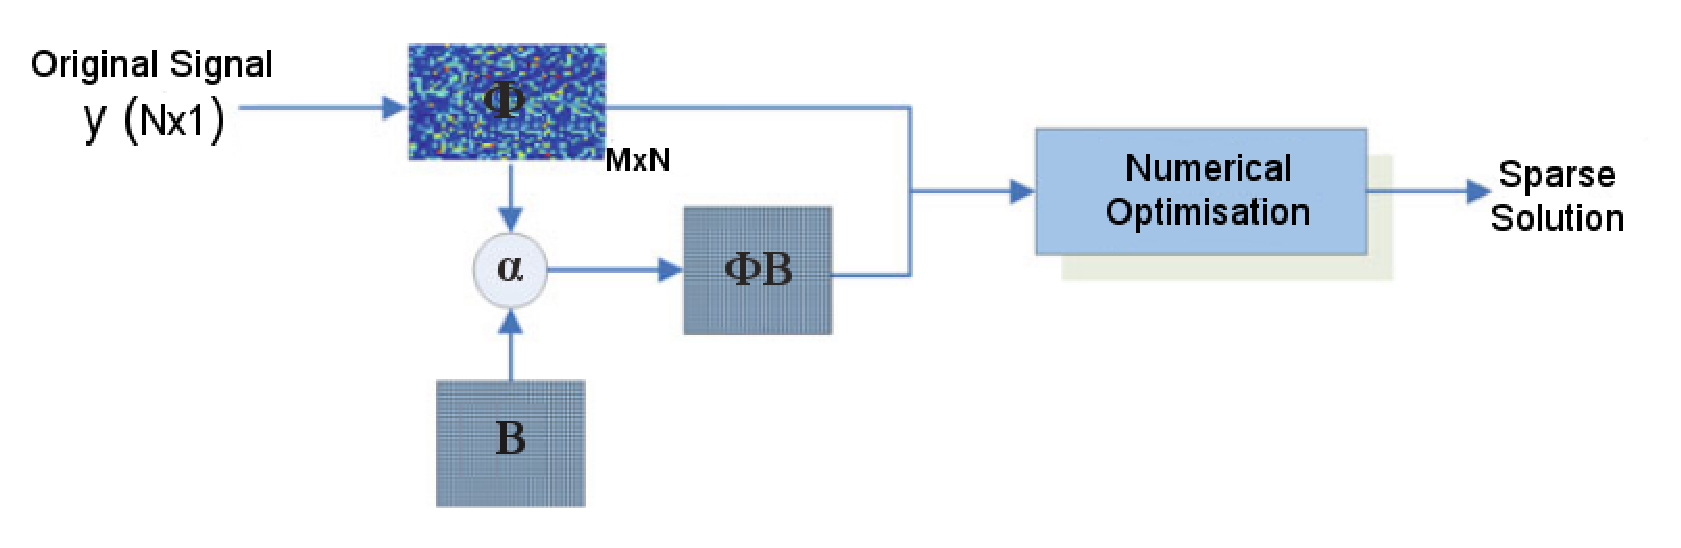
\includegraphics[width=\textwidth]{images/sparse.eps}
\caption[Proceso de \textit{Compressed sensing}]{Proceso de \textit{Compressed sensing} \cite{compressive}}
\label{fig:compressive}
\end{figure}












\clearpage\chapter{Estado del Arte}
\label{chap:related}

\section{Entrenamiento de Diccionarios}

Uno de los elementos fundamentales para el CS es la selecci\'on del diccionario, ya que con un buen diccionario se pueden garantizar una mejor reconstrucci\'on de una se\~nal. Para la seleci\'on del diccionario se pueden usar muestras extraidas directamente de la se\~nal que se debe reconstruir o de una se\~nal con caracter\'isticas similares, o se puede realizar un entrenamiento del diccionario para que se adapte a las condiciones de la se\~nal \cite{dictionaries}. A continuaci\'on se presenta una revisi\'on de los prinicpales algoritmos de entrenamiento. 

\subsection{M\'etodo de direcciones \'optimas }
El M\'etodo de Direcciones \'Optimas (MOD) fue propuesto por Eagan \textit{et al.} en 1999 \cite{omp} para fines de compresi\'on de se\~nales. Los principales pasos del algoritmo MOD son:
\begin{enumerate}
\item Inicialmente se tienen un $\bm{y}_i$, $i=1,2, .., K$ como conjunto de entrenamiento, un $\bm{D}_0$ de tama\~no $N \times M$ y un contador $c = 1$ 
\item Se aproxima cada vector de entrenamiento $\bm{y}_i$, usando un algoritmo para seleccionar el vector disperso 
\begin{equation}
\bm{\widetilde{y}}_i=\bm{Dx} = \sum \limits_{j=1}^{M} \bm{x}_i(j) \bm{d}_j
\end{equation}
donde $\bm{x}_i(j)$ es el coeficiente correspondiente al vector $\bm{d}_j$. Una vez se obtiene la aproximaci\'on $\bm{\widetilde{y}}_i$, se calculan los valores residuales entre la aproximaci\'on y la se\~nal original
\item \label{new} Dadas las aproximaciones y el residual, se calcula un nuevo diccionario $\bm{D}_i$ usando los vectores \'optimos $\bm{\delta}_i$ en
\begin{equation}
\bm{\widetilde{D}}_i= \bm{D}_i + \bm{\delta}_i
\end{equation}
\item Se vuelven a calcular nuevas aproximaciones y residuales, si no se cumple la condici\'on de parada se actualiza el contador $c = c + 1$ y se realiza de nuevo el paso \ref{new}. Los criterios de parada pueden ser un n\'umero de iteraciones o una restricci\'on en el residual.
\end{enumerate}

Dado que la soluci\'on del problema del vector disperso es NP-Hard, solo se puede hallar una soluci\'on aproximada con la desventaja de caer en m\'inimos locales.  

\subsection{K-SVD}
El algoritmo de aprendizaje K-SVD es una generalizaci\'on del algortimo K-means mediante descomposici\'on en valores singulares (SVD) y fue propuesto por Elad \textit{et al.} en 2005 \cite{k-svd}. El K-SVD, al igual que el MOD, realiza un proceso de selecci\'on del vector disperso y uno de actualizaci\'on del diccionario, con la diferencia que la actualizaci\'on se realiza por \'atomos del diccionario y no en su totalidad. El K-SVD busca representar una muestra $\bm{y}_i$ resolviendo una funci\'on objetivo mediante los siguientes pasos:
\begin{enumerate}
\item Inicialmente se tiene un diccionario $\bm{D}_0$ y una variable de conteo $j=1$
\item \label{alg:ksvd} Usando alg\'un algoritmo de selecci\'on de vector disperso, basado en la norma $\ell_0$ o $\ell_1$, se calcula $\bm{x}_i$ para cada muestra $\bm{y}_i$, aproximando la soluci\'on a
\begin{equation}
\min_{\bm{x}_i}\{||\bm{y}_i-\bm{Dx}_i||_2^2\}\;\; \text{sujeto a} \;\; \forall_i, ||\bm{x}_i||_0 \leq T_0 
\end{equation}
donde $T_0$ es un valor de error en la aproximaci\'on
\item Cada \'atomo $K = 1,2,...,N$ en $D_{j-1}$ es actualizado por el siguiente algoritmo:
\begin{itemize}
\item Se define un conjunto de muestras que usan ese \'atomo, $ \omega_i = \{ i|1 \leq i \leq N, \bm{x}_T^k(i) \neq 0\}$
\item Se calcula el error de la $E_k$ mediante
\begin{equation}
E_k = \bm{y}-\sum \limits_{j\neq k} \bm{d}_j \bm{x}_T^j
\end{equation}
\item Se rentringue $E_k$ seleccionando solo las columnas que corrsponden a $\omega_k$
\item Se aplica la descomposici\'on en valores singulares de $E_T^R = U\Delta V^T$. Se selecciona la columna $\widetilde{\bm{d}}_k$ para ser la primera columna de $U$ y se actualiza la vector de coeficiente $\bm{x}_R^k$ como primer columna de $V$ multiplicado por $\Delta (1,1)$
\end{itemize}
\item Si no se cumple el criterio de parada se incrementa el contador $j = j+1$ y se retorna al paso \ref{alg:ksvd}. 
\end{enumerate}
Al igual que el MOD, el K-SVD presenta problemas de m\'inimos locales, pero la actualizaci\'on por \'atomos le permite que el proceso de entrenamiento sea m\'as r\'apido.

\subsection{Algoritmo de Aprendizaje en linea}
El algoritmo de entranamiento en linea fue propuesto por Mairal \textit{et al.} en 2010 \cite{online} y se basa en aproximaciones estoc\'asticas. El algoritmo en linea se describe a continuaci\'on:
\begin{enumerate}
\item Inicialmente se tiene un diccionario $\bm{D}_0$, un n\'umero $j$ de iteraciones y un par\'ametro de regularizaci\'on $\lambda$
\item Se crean las matrices $\bm{A} \in \mathbb{R}^{K \times K}$ y  $\bm{B} \in \mathbb{R}^{M \times K}$ y se inicializan con valor 0
\item Se toman muestras de $\bm{y}_j$ basados en una distribuci\'on de probabilidad $p$
\item Se halla el vector disperso usando el algoritmo de regersi\'on de menor \'angulo (LARS) \cite{lars}
\begin{equation}
\min_{\bm{x}_k} \frac{1}{2}||\bm{y}_j-\bm{D}_{j-1}\bm{x}||^2_2+\lambda||\bm{x}||_1
\end{equation}
\item Se asignan valores a las matrices $\bm{A}_j = \bm{A}_{j-1}+\bm{x}_j\bm{x}_j^T$ y $\bm{B}_j = \bm{B}_{j-1}+\bm{y}_j\bm{x}_j^T$ 
\item Se calcula $\bm{D}_j$ actualizando la columna $j$ desde $j=1$ hasta $j=k$ teniendo en cuenta que $\bm{D} =[\bm{d}_1, \ldots, \bm{d}_k]$, $\bm{A} =[\bm{a}_1, \ldots, \bm{a}_k]$ y $\bm{B} =[\bm{b}_1, \ldots, \bm{b}_k]$. Este proceso se realiza hasta que converja hasta un l\'imite
\begin{align}
\bm{u}_j &= \frac{1}{\bm{A}_{jj}}(\bm{b}_j - \bm{Da}_j) + \bm{d}_j, \\
\bm{d}_j &= \frac{1}{\max(||\bm{u}_j||_2, 1)\bm{u}_j}
\end{align}
\item Luego $\bm{D}_j$ es calculado usando
\begin{align}
\bm{D}_j &= \min_{\bm{D}} \frac{1}{t}\sum \limits_{i=1}^j\frac{1}{2}||\bm{y}_i-\bm{Dx}_i||_2^2+\lambda||\bm{x}||_1
\end{align}
\end{enumerate}

Este algoritmo funciona bien para grandes cantidades de datos ya que se actualiza gradualmente mientras se esperan otros datos.

\section{Codificaci\'on de video usando Compressed Sensing}
\label{sec:codificacion_dispersa}
Uno de los enfoques de la CS es la compresi\'on de se\~nales. En el caso del video, se integran las t\'ecnicas de CS con los procesos involucrados en la codificaci\'on de video para representar la informaci\'on con una cantidad menor de muestras. Para obtener el diccionario, en algunos casos se seleccionan directamente bloques de la imagen con ciertas caracter\'isticas  y en otros se aplican algoritmos de entrenamiento del diccionario. Inicialmente se trabajaban con diccionarios preseleccionados debido a la complejidad que involucraba el entrenamiento, por ejemplo  Stankovic \textit{et al.}, en una de las primeras propuestas de CS en video \cite{stankovic2008compressive}, integran las t\'ecnicas de CS para representar los frames que no son im\'agenes de referencia evaluando la dispersi\'on del frame de referencia. Como diccionario se selecciona una combinaci\'on de una matriz aleatoria de distribuci\'on gausiana y la transformada discreta del coseno (DCT) de cada bloque. La DCT de cada bloque del frame de referencia se compara con una constante, y si el valor es mayor, todos los bloques co-localizados en los frames que no son de referencia son muestreados compresivamente usando el algoritmo de correspondencias ortogonales.  

En \cite{do2009distributed}, Do \textit{et al.} combinan los conceptos de CS con la codificaci\'on de video distribuida, donde se translada la complejidad de la codificaci\'on al lado del decodificador. En el codificador se seleccionan frames claves, que son codificados con m\'etodos tradicionales, y los frames no claves que son codificados explotando la dispersion en la predicci\'on inter-frame y recuperando la informaci\'on dispersa en el decodificador. Como muestras para construir el diccionario se usan los bloques vecinos co-localizados en los frames clave. Cheng \textit{et al.} realizan una propuesta similar en \cite{chen2010dictionary}, con la diferencia de que el diccionario es entrenado usando el algoritmo K-SVD. 

En \cite{haixiao_dictionary_2011}, Haixiao \textit{et al.} usan el proceso de estimaci\'on de movimiento para el entrenamiento del diccionario. El diccionario es inicializado usando bloques transformados de la imagen de referencia y la actualizaci\'on del diccionario se realizan estimando la reconstrucci\'on del frame actual mediante la compensaci\'on de movimiento. La evaluaci\'on del diccionario se realiza por medio de cada unidad de codificaci\'on que compone la imagen. Tambi\'en
se debe tener en cuenta un proceso de filtrado para remover artefactos de bloques en las im\'agenes y mejorar la calidad en la imagen reconstruida.

En \cite{kang_efficient_2011}, Kang \textit{et al.} proponen un modelo para entrenar el diccionario con los residuales de las muestras predecidas. Estas muestras deben ser clasificicadas de acuerdo al contexto ya que todas no pueden ser usadas para el entrenamiento. La clasificaci\'on es realizada mediante caracter\'isticas espec\'ificas de las muestras como la direcci\'on en la predicci\'on intra-frame o la energ\'ia gastada en codificaci\'on para la predicci\'on inter-frame. Como algoritmo de entrenamiento se usa el K-SVD  y para transmitir el diccionario al decodificador se usa un \'indice del diccionario con una bandera que indica de cual vecino es copiado, de esta forma solo se transmiten los coeficientes que cambian respecto al vecino.

En \cite{wahidah_compressive_2012}, Wahidah \textit{et al.} proponen un modelo de codificaci\'on de video usando la dispersi\'on din\'amica de la fuente, modelando la se\~nal de video en el dominio disperso usando la DCT o la transformada de \textit{wavelet}. La din\'amica de la escena es medida con el n\'umero de coeficientes no significativos y se establece un umbral con un valor peque\~no para tomar una menor cantidad de coeficientes. El modelo propuesto usa un diccionario predefinido y por cada imagen en el grupo de im\'agenes se eval\'ua si es v\'alido como frame disperso, de lo contrario se codifica con m\'etodos tradicionales.  

En \cite{xiong2013sparse}, Xiong \textit{et al.} proponen un modelo de aprendizaje adaptativo regularizado para esquemas de codificaci\'on de video con bajas tasas de bits. El modelo propuesto selecciona  frames claves que son codificados en resoluci\'on original mientras el resto son codificados en una version de baja resoluci\'on del frame y son reconstruidos mediante la representaci\'on dispersa  de los frames claves, entrenando los diccionarios con el algoritmo K-SVD teniendo en cuenta los cambios temporales y espaciales de las muestras.

En \cite{sun2012online}, Sun \textit{et al.} proponen el aprendizaje del diccionario desde frames previos para codificar  el video mediante la representaci\'on dispersa de los frames que llegan a codificar. El diccionario es inicializado con bloques de la imagen los cuales han sido transformados usando la DCT. El diccionario se entrena mediante el algoritmo de entramiento en linea y se actualiza cada cierta cantidad de im\'agenes. Para sincronizar el diccionario con el decodificador se envia el residual entre el diccionario actualizado y el diccionario previo.

En \cite{song_omp-based_2016}, Song \textit{et al.} proponen un un diccionario adaptativo para el proceso de transformaci\'on en el HEVC usando el algoritmo de b\'usqueda de correspondencias ortogonales. La construcci\'on del diccionario se realiza explotando las correlaciones no locales a partir de regiones reconstruidas (predicci\'on inter-frame), en este caso el diccionario no es entrenado. Los bloques para el diccionario se seleccionan basados en el residual de la compensaci\'on de movimiento.

Dai \textit{et al.} proponen en \cite{dai_sparse_2016} un algoritmo para aumentar la convergencia del aprendizaje del diccionario incorporando un gradiente descendente estoc\'astico. Esta propuesta maneja el mismo principio de baja y alta resoluci\'on de \cite{xiong2013sparse} pero el diccionario es entrenado usando el entrenamiento en linea.  

He \textit{et al.} proponen en \cite{he_improvement_2016} reemplazar la predicci\'on intra-frame, calculando el mapeo
contractivo disperso para aproximar el frame intra y el siguiente frame con predicci\'on inter-frame, y eliminando los bloques de frames intra, basados en errores de aproximaci\'on producidos en el mapeo contractivo. En esta propuesta el diccionario  es construido usando trozos de la imagen que son rotados o con bloques generados por las direcciones de la predicci\'on intra.

\section{Codificaci\'on de video perceptual}
\label{sec:codificacion_perceptual}

Las t\'ecnicas de codificaci\'on de video perceptual tienen en cuenta caracter\'isticas del HVS como punto final del proceso de codificaci\'on. Dentro de las caracter\'isticas que tienen en cuenta se encuentran la sensitividad al contraste, donde un est\'imulo no es visto por su frecuencia, el enmascaramiento, donde un est\'imulo reduce la visibilidad de otro est\'imulo, la fovea que indica el \'angulo de visi\'on del ojo humano y la atenci\'on visual que indica los aspectos particulares donde se enfoca la visi\'on \cite{perceptual}. Los modelos de codificaci\'on perceptual buscan explotar estas condiciones para darle una mayor importancia a ciertas regiones de las im\'agenes del video.

\subsubsection{Regiones de inter\'es}

Las regiones de inter\'es buscan detectar zonas de los frames de video donde se debe mantener alto nivel de calidad. Las regiones de inter\'es pueden ser definidas por el usuario o pueden ser detectadas autom\'aticamente. En \cite{meddeb2014region}, Meddeb \textit{et al.} proponen un modelo para asignar una mayor cantidad de bits a regiones de inter\'es para sistemas de video conferencia. El algoritmo detecta autom\'aticamente regiones de inter\'es, que son principalmente rostros. En \cite{6782435}, Xu \textit{et al.} proponen un modelo de percepci\'on jer\'arquico de detecci\'on de rostros para video conversacional. En este modelo se da una ponderaci\'on a cada componente del rostro (ojos, labios entre otros).

\subsubsection{Distorsi\'on apenas notable}
La distori\'on apenas notable (JND) aprovecha los mecanismos de enmascaramiento del HVS, que se refiere al m\'aximo nivel distorsi\'on que no se puede percibir y que se encuentra bajo un umbral de sensitividad visual. Con estos mecanismos las regiones donde la distortsi\'on es m\'as notable tienen una mayor importancia. Kim \textit{et al.} presentan en \cite{kim_hevc-compliant_2015} un modelo JND en el dominio de los pixeles para transformar el modo \textit{skip} del HEVC en el dominio de la transformada. Como caracter\'isticas espaciales en el dominio de la transformada se tienen en cuenta la sensitividad al contraste, la adaptaci\'on a la luminancia y los efectos de enmascaramiento del contraste.

\subsubsection{Saliencia visual}
La saliencia representa la probabilidad de que el HVS preste atenci\'on a ciertos objetos del frame en lugar de otros. La saliencia es representada en un mapa, generalmente en escala de grises, donde se muestra la ubicaci\'on de los objetos con respecto a sus vecinos. En \cite{saliency}, Wei \textit{et al.} construyen el mapa de saliencia usando un algoritmo basado en la estructura local de los datos, calculado mediante un kernel de direcci\'on local, y  una medida de auto-semejanza. En \cite{wang_perceptual_2014} propone un modelo que combine el modelo de atenci\'on visual y el modelo de sensitividad visual. Para este modelo se expresa la imagen como un producto de un pixel en el dominio de JND y un factor de modulaci\'on de saliencia. Para el modelo JND espacial se establece un umbral despu\'es de aplicar la DCT a los bloques de la imagen.

\section{Codificaci\'on de Video usando Representaci\'on Dispersa y Codificaci\'on Perceptual}
\label{sec:codificacion_dispersa_perceptual}

Algunas propuestas se basan en las t\'ecnicas de CS para codificaci\'on de video teniendo en cuenta las caracter\'isticas perceptuales del HVS. En \cite{elsayed_perceptual-based_2015} proponen dos frameworks, uno que se encargue de la predicci\'on intra-frame y otro que se encargue de la predicci\'on inter-frame. En la predicci\'on intra-frame las im\'agenes son adquiridas y recuperadas cada una por separado, mientras en la predicci\'on inter-frame, las im\'agenes son adquiridas y recuperdas basadas en la correlaci\'on que tienen con im\'agenes de referencia utilizando el residual. Como medida de percepci\'on para el c\'alculo de la representaci\'on dispersa de la se\~nal se usan las frecuencias m\'as bajas en el dominio
de la DCT. Tambi\'en se usa una ponderaci\'on est\'atica para explotar regiones con baja frecuencia. En esta propuesta el diccionario es contruido con los coeficientes de la DCT ponderados mediante una matriz de pesos. Xu \textit{et al.} proponen en \cite{xu_perceptually-aware_2015} un modelo basado en la estimaci\'on de la correlaci\'on del ruido entre un frame no clave y su representaci\'on en el codificador y explotando la interpolaci\'on de los bloques que usan compensaci\'on de movimiento con lo cual se obtiene la correlaci\'on temporal entre frames reconstruidos en el lado de la informaci\'on. Con esta informaci\'on se calcula la saliencia espacial y temporal de los bloques de la imagen para definir cuales pueden ser reconstruidos usando CS. 





\clearpage% Bibliography

\label{app:bibliography} % Reference the bibliography elsewhere with \autoref{app:bibliography}

\manualmark
\markboth{\spacedlowsmallcaps{\bibname}}{\spacedlowsmallcaps{\bibname}} 
\refstepcounter{dummy}

\addtocontents{toc}{\protect\vspace{\beforebibskip}} % Place the bibliography slightly below the rest of the document content in the table of contents
\addcontentsline{toc}{chapter}{\tocEntry{\bibname}}

\bibliographystyle{ieeetr}

\bibliography{Bibliography}

\end{document}